%File: anonymous-submission-latex-2024.tex
\documentclass[letterpaper]{article} % DO NOT CHANGE THIS
\usepackage[submission]{aaai24}  % DO NOT CHANGE THIS
\usepackage{times}  % DO NOT CHANGE THIS
\usepackage{helvet}  % DO NOT CHANGE THIS
\usepackage{courier}  % DO NOT CHANGE THIS
\usepackage[hyphens]{url}  % DO NOT CHANGE THIS
\usepackage{graphicx} % DO NOT CHANGE THIS
\urlstyle{rm} % DO NOT CHANGE THIS
\def\UrlFont{\rm}  % DO NOT CHANGE THIS
\usepackage{natbib}  % DO NOT CHANGE THIS AND DO NOT ADD ANY OPTIONS TO IT
\usepackage{caption} % DO NOT CHANGE THIS AND DO NOT ADD ANY OPTIONS TO IT
\frenchspacing  % DO NOT CHANGE THIS
\setlength{\pdfpagewidth}{8.5in} % DO NOT CHANGE THIS
\setlength{\pdfpageheight}{11in} % DO NOT CHANGE THIS
%
% These are recommended to typeset algorithms but not required. See the subsubsection on algorithms. Remove them if you don't have algorithms in your paper.
\usepackage{algorithm}
\usepackage{algpseudocode}

%New Package
\usepackage{tablefootnote}
\usepackage{mathtools}
\usepackage{amsfonts}
\usepackage{multirow}
\usepackage{multicol}
\usepackage{booktabs}
\usepackage[dvipsnames]{xcolor}
\usepackage{adjustbox}
\setcounter{table}{3}
\setcounter{figure}{5}
\usepackage{makecell}
\usepackage{supertabular}
%
% These are are recommended to typeset listings but not required. See the subsubsection on listing. Remove this block if you don't have listings in your paper.
\usepackage{newfloat}
\usepackage{listings}
\DeclareCaptionStyle{ruled}{labelfont=normalfont,labelsep=colon,strut=off} % DO NOT CHANGE THIS
\lstset{%
	basicstyle={\footnotesize\ttfamily},% footnotesize acceptable for monospace
	numbers=left,numberstyle=\footnotesize,xleftmargin=2em,% show line numbers, remove this entire line if you don't want the numbers.
	aboveskip=0pt,belowskip=0pt,%
	showstringspaces=false,tabsize=2,breaklines=true}
\floatstyle{ruled}
\newfloat{listing}{tb}{lst}{}
\floatname{listing}{Listing}
%
% Keep the \pdfinfo as shown here. There's no need
% for you to add the /Title and /Author tags.
\pdfinfo{
/TemplateVersion (2024.1)
}

% DISALLOWED PACKAGES
% \usepackage{authblk} -- This package is specifically forbidden
% \usepackage{balance} -- This package is specifically forbidden
% \usepackage{color (if used in text)
% \usepackage{CJK} -- This package is specifically forbidden
% \usepackage{float} -- This package is specifically forbidden
% \usepackage{flushend} -- This package is specifically forbidden
% \usepackage{fontenc} -- This package is specifically forbidden
% \usepackage{fullpage} -- This package is specifically forbidden
% \usepackage{geometry} -- This package is specifically forbidden
% \usepackage{grffile} -- This package is specifically forbidden
% \usepackage{hyperref} -- This package is specifically forbidden
% \usepackage{navigator} -- This package is specifically forbidden
% (or any other package that embeds links such as navigator or hyperref)
% \indentfirst} -- This package is specifically forbidden
% \layout} -- This package is specifically forbidden
% \multicol} -- This package is specifically forbidden
% \nameref} -- This package is specifically forbidden
% \usepackage{savetrees} -- This package is specifically forbidden
% \usepackage{setspace} -- This package is specifically forbidden
% \usepackage{stfloats} -- This package is specifically forbidden
% \usepackage{tabu} -- This package is specifically forbidden
% \usepackage{titlesec} -- This package is specifically forbidden
% \usepackage{tocbibind} -- This package is specifically forbidden
% \usepackage{ulem} -- This package is specifically forbidden
% \usepackage{wrapfig} -- This package is specifically forbidden
% DISALLOWED COMMANDS
% \nocopyright -- Your paper will not be published if you use this command
% \addtolength -- This command may not be used
% \balance -- This command may not be used
% \baselinestretch -- Your paper will not be published if you use this command
% \clearpage -- No page breaks of any kind may be used for the final version of your paper
% \columnsep -- This command may not be used
% \newpage -- No page breaks of any kind may be used for the final version of your paper
% \pagebreak -- No page breaks of any kind may be used for the final version of your paperr
% \pagestyle -- This command may not be used
% \tiny -- This is not an acceptable font size.
% \vspace{- -- No negative value may be used in proximity of a caption, figure, table, section, subsection, subsubsection, or reference
% \vskip{- -- No negative value may be used to alter spacing above or below a caption, figure, table, section, subsection, subsubsection, or reference

\setcounter{secnumdepth}{0} %May be changed to 1 or 2 if section numbers are desired.

% The file aaai24.sty is the style file for AAAI Press
% proceedings, working notes, and technical reports.
%

% Title

% Your title must be in mixed case, not sentence case.
% That means all verbs (including short verbs like be, is, using,and go),
% nouns, adverbs, adjectives should be capitalized, including both words in hyphenated terms, while
% articles, conjunctions, and prepositions are lower case unless they
% directly follow a colon or long dash
\title{AAAI Press Anonymous Submission\\Instructions for Authors Using \LaTeX{}}
\author{
    %Authors
    % All authors must be in the same font size and format.
    Written by AAAI Press Staff\textsuperscript{\rm 1}\thanks{With help from the AAAI Publications Committee.}\\
    AAAI Style Contributions by Pater Patel Schneider,
    Sunil Issar,\\
    J. Scott Penberthy,
    George Ferguson,
    Hans Guesgen,
    Francisco Cruz\equalcontrib,
    Marc Pujol-Gonzalez\equalcontrib
}
\affiliations{
    %Afiliations
    \textsuperscript{\rm 1}Association for the Advancement of Artificial Intelligence\\
    % If you have multiple authors and multiple affiliations
    % use superscripts in text and roman font to identify them.
    % For example,

    % Sunil Issar\textsuperscript{\rm 2},
    % J. Scott Penberthy\textsuperscript{\rm 3},
    % George Ferguson\textsuperscript{\rm 4},
    % Hans Guesgen\textsuperscript{\rm 5}
    % Note that the comma should be placed after the superscript

    1900 Embarcadero Road, Suite 101\\
    Palo Alto, California 94303-3310 USA\\
    % email address must be in roman text type, not monospace or sans serif
    proceedings-questions@aaai.org
%
% See more examples next
}

%Example, Single Author, ->> remove \iffalse,\fi and place them surrounding AAAI title to use it
\iffalse
\title{My Publication Title --- Single Author}
\author {
    Author Name
}
\affiliations{
    Affiliation\\
    Affiliation Line 2\\
    name@example.com
}
\fi

\iffalse
%Example, Multiple Authors, ->> remove \iffalse,\fi and place them surrounding AAAI title to use it
\title{My Publication Title --- Multiple Authors}
\author {
    % Authors
    First Author Name\textsuperscript{\rm 1},
    Second Author Name\textsuperscript{\rm 2},
    Third Author Name\textsuperscript{\rm 1}
}
\affiliations {
    % Affiliations
    \textsuperscript{\rm 1}Affiliation 1\\
    \textsuperscript{\rm 2}Affiliation 2\\
    firstAuthor@affiliation1.com, secondAuthor@affilation2.com, thirdAuthor@affiliation1.com
}
\fi


% REMOVE THIS: bibentry
% This is only needed to show inline citations in the guidelines document. You should not need it and can safely delete it.
\usepackage{bibentry}
% END REMOVE bibentry

\begin{document}

\section{Technical Appendix}
For a better understanding, we provide auxiliary resources regarding our proposed EIISRS model in the appendix, including algorithm, complexity analysis, additional case studies, and notations.
\section{A{\quad}Algorithm}
\begin{algorithm}[h]
    \caption{The first training epoch of EIISRS}
    \label{alg:algorithm}
    \textbf{Input}: user-item interaction matrix $\textbf{\textit{R}}$, social networks $\textbf{\textit{S}}$, and Gaussian random initialize user embeddings $\textbf{\textit{P}}^{(0)}$ and item embeddings $\textbf{\textit{Q}}^{(0)}$\\
    \textbf{Output}: user embeddings $\textbf{\textit{P}}_{final}$ and item embeddings $\textbf{\textit{Q}}$, augmented social networks $\widetilde{\textbf{\textit{S}}}$
    \begin{algorithmic}[1]
        \For{each epoch}
            \For{each batch}
                \State $\textbf{\textit{P}}^{(0)}_s, \textbf{\textit{P}}^{(0)}_r \gets$ Eq.(1); \textcolor{RoyalBlue}{\small\Comment{Self-gating Unit}}
                \For{$l=1:L$}
                    \State $\textbf{\textit{P}}^{(l)}_s$, $\textbf{\textit{P}}^{(l)}_r$, $\textbf{\textit{Q}}^{(l)}$ $\gets$ Eq.(2)-(4);\textcolor{RoyalBlue}{\small\Comment{Graph Conv.}}
                    \State $\boldsymbol{\mu}^{(l)}$, $\boldsymbol{\sigma}^{(l)} \gets$ Eq.(8);
                    \State $\textbf{\textit{Z}}_s^{(l)} \gets$ Eq.(9); \textcolor{RoyalBlue}{\small\Comment{Social Diversity Simulation}}
                    \State ${\alpha}_l \gets$ Eq.(5);
                    \State Calculate the $\mathcal{L}_{reconstruct}$ and $KLD$;
                \EndFor
                \State $\widetilde{\textbf{\textit{P}}}_s = \sum_{i=0}^{L}\alpha_l\textbf{\textit{Z}}_s^{(l)}$; \textcolor{RoyalBlue}{\small\Comment{Social Influence Propagation}}
                \State $\textbf{\textit{P}}_{final} \gets$ Eq.(14);
                \State Calculate the pairwise BPR loss $\mathcal{L}_{rec}$;
            \EndFor
            \State $\widetilde{\textbf{\textit{S}}} \gets$ Eq.(10)-(13); \textcolor{RoyalBlue}{\small\Comment{Social Influence Exploration}}
        \EndFor
        \State return $\textbf{\textit{P}}_{final}, \textbf{\textit{Q}}, \widetilde{\textbf{\textit{S}}}$
    \end{algorithmic}
\end{algorithm}
For the remaining training epochs, we replace the social networks \textbf{\textit{S}} with augmented social networks $\widetilde{\textbf{\textit{S}}}$ as input.

\section{B{\quad}Complexity Analysis}
This section elaborates on the model size and time complexity of our model.
\subsection{Model Size}
For model size, there are six parts that introduce trainable parameters: user/item embeddings, self-gating units, layerwise attention unit, selectors, encoder/decoder in LGE-VAE, and aggregation matrix. The size of user and item embeddings in total is $(m+n)\times d$. Each self-gating unit and layerwise attention unit occupies $(d+1)\times d$, altogether $3\times (d+1)$. $K$ selectors take up $k\times m$ in total. Encoder occupies $2\times d\times d$ while decoder is $d\times d$, same as the aggregation matrix. To sum up, the total size of our model is approximately equal to $(m+n+7d+3)\times d+ k\times m$. Since $d\ll min(m,n)$ and $k\ll m$, we can conclude that our model is fairly portable.
\subsection{Time Complexity}
For time complexity, analogously, there are also the six parts that cost our computational power. Regarding graph convolution, the time complexity is $\mathcal{O}(|\textbf{\textit{R}}^+|dL)$ for the user-item bipartite graph, and $\mathcal{O}(|\textbf{\textit{S}}^+|dL)$ for the social graph, where $|\textbf{\textit{R}}^+|$ and $|\textbf{\textit{S}}^+|$ denote the non-zero values of original graphs respectively. Compared with previous graph-based recommendation systems, we drop the feature transformation matrix and activation function, so the time complexity of graph convolution is relatively slower. For the self-gating units, layerwise attention unit, encoder/decoder of LGE-VAE, and aggregation matrix, the time complexity is as low as $\mathcal{O}(md^2)$. As for the selector, it could incur massive time consumption if we need to calculate the cosine similarity among all users, since the time complexity would be $\mathcal{O}(m^2d)$ and would exponentially increase along with the linear increment of our input data. To tackle this problem, for each epoch, we only choose a tiny subset of users $\mathcal{U}^+$ to do the processing, in which $|\mathcal{U}^+| \ll m$. After the two most time-consuming components, namely graph convolution and selectors, have been tailored without spoiling the effectiveness, our model is fairly efficient, too.

\section{C{\quad}Case Study}
This section exhibits some case studies of our model as supplements, in order to illustrate the validity of our hypothesis. For simplicity, we take LastFM as the only dataset to implement the visualization analysis experiments. 
\subsection{Analysis of Implicit Social Graph}
\begin{figure}[ht!]
  \centering
  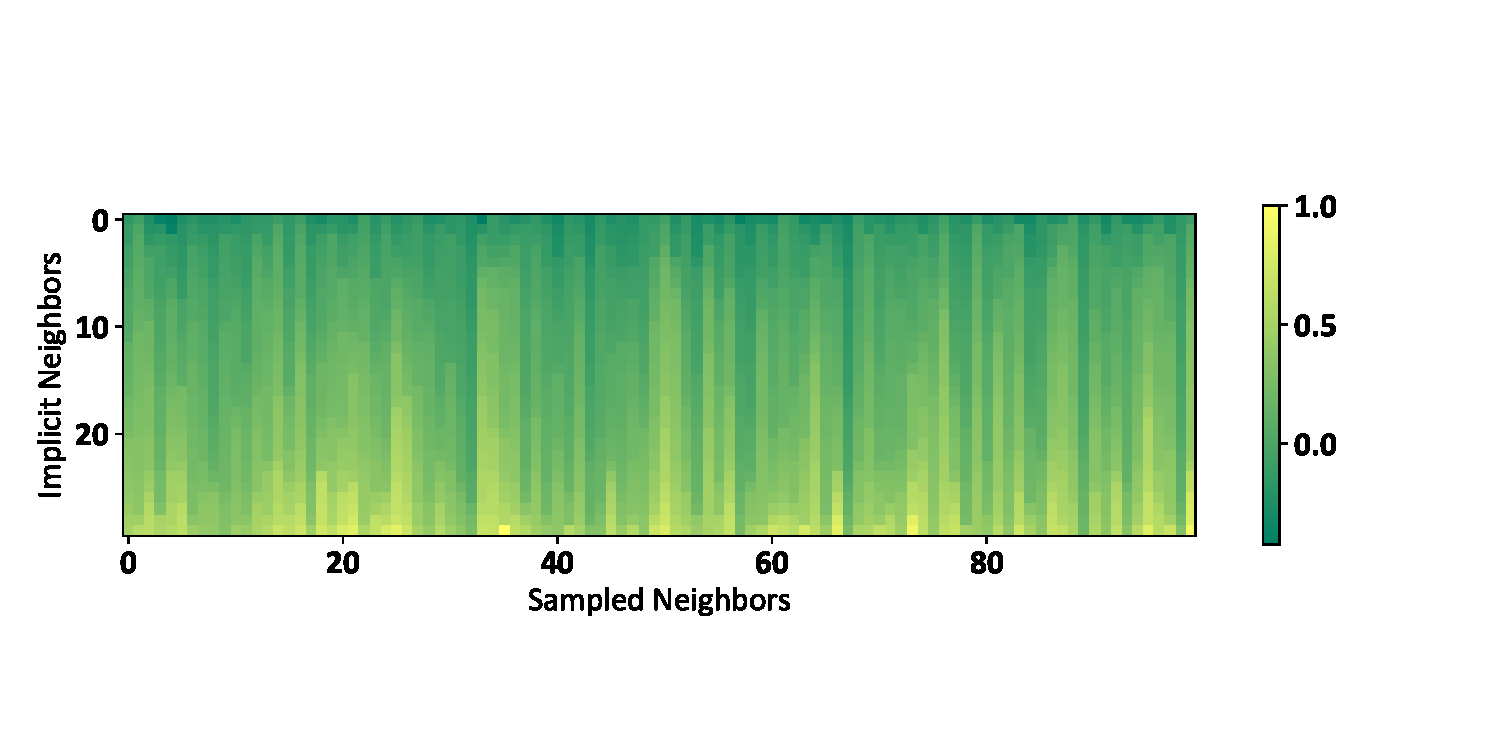
\includegraphics[width=0.5\textwidth]{implicit.pdf} %1.png是图片文件的相对路径
  \caption{Illustration of the similarity with implicit social neighbors.}
  \label{fig_implicit}
\end{figure}
\noindent As shown in Figure \ref{fig_implicit}, the color shows the similarity between sampled neighbors and generated implicit neighbors. The closer the score to 1, the more similar the two users are, and the lighter the color is. Vice versa. We can observe from the graph that different candidate neighbors have different similarities. We can make an inference that the implicit neighbors are not always highly similar to the sampled user since the anchor user probably has diverse interests and cannot be exactly assigned to an agminated neighborhood. It is also evidence of why we apply social diversity simulation in our model.

\begin{figure*}[ht]
  \centering
  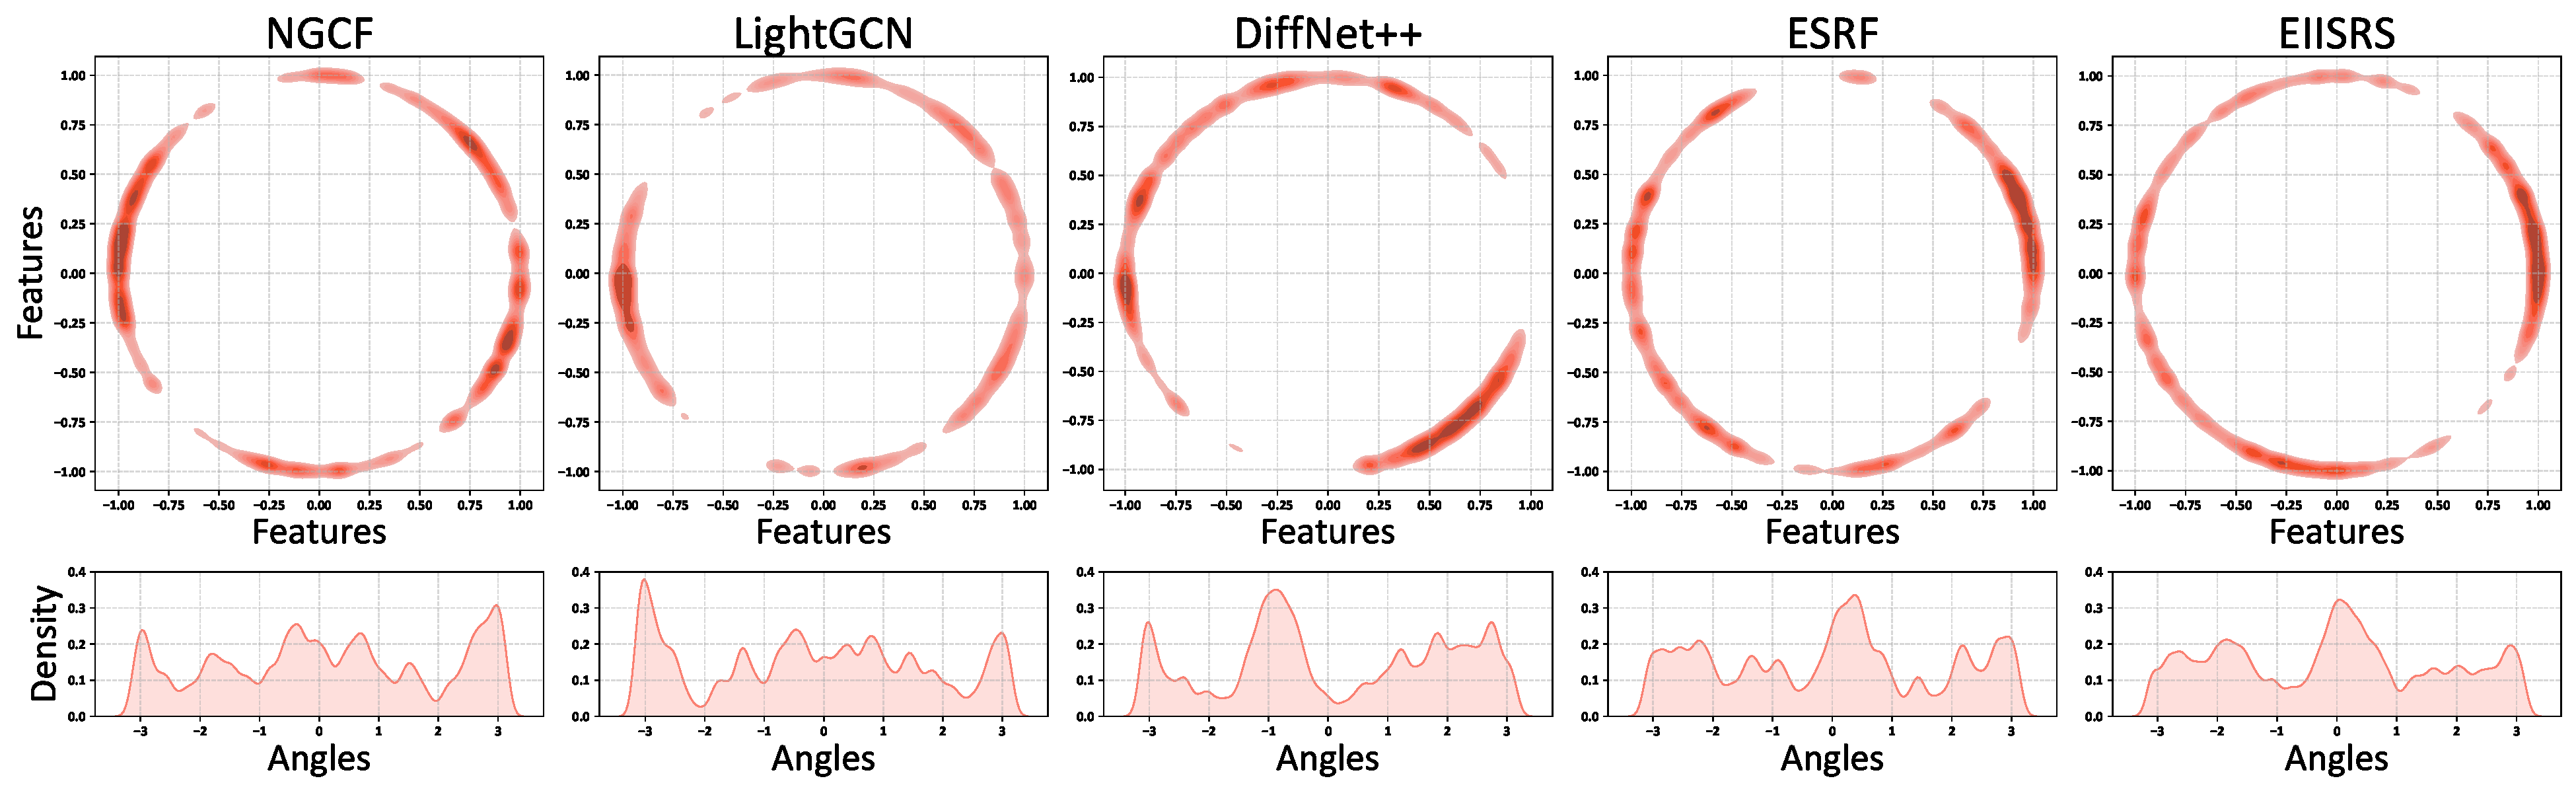
\includegraphics[width=1.02\textwidth]{tsne.pdf} %1.png是图片文件的相对路径
  \caption{Visualization of user representations on LastFM. }
  \label{fig_tsne}
\end{figure*}

% \begin{table*}[ht]\small
%     \centering
%     \flushleft
%     \begin{tabular*}{\textwidth}{@{\extracolsep{\fill}}ccccc|cccc|cccc}
%         \cmidrule(l){1-13}
%         \multirow{2}{*}{Model} & \multicolumn{4}{c}{LastFM} & \multicolumn{4}{c}{Flickr} & \multicolumn{4}{c}{Yelp} \\ \cmidrule(l){2-5} \cmidrule(l){6-9} \cmidrule(l){10-13} \cmidrule(l){10-13}
%             & P@10  & R@10  & F1@10  & N@10 & P@10  & R@10 & F1@10  & N@10 & P@10 & R@10 & F1@10  & N@10 \\ \cmidrule(l){1-13}
%             SGL             &0.0911 &0.1848 &0.1220 &0.1708     &0.0019 &0.0042 &0.0026 &0.0034     &0.0033 &0.0276 &0.0059 &0.0145\\
            
%             NCL            &0.0944 &0.1934 &0.1269 &0.1880     &0.0019 &0.0049 &0.0027 &0.0041     &0.0034 &0.0277 &0.0061 &0.0137\\ \cmidrule(l){1-13}
            
%             SEPT        &0.1889 &0.1911 &0.1900 &0.2459     &\textbf{0.0038} &0.0042 &0.0040 &0.0047     &0.0061 &0.0239 &0.0097 &0.0148 \\

%             MHCN        &\textbf{0.1961} &\underline{0.1994} &\underline{0.1977} &\textbf{0.2547}    &\underline{0.0036} &\textbf{0.0050} &\textbf{0.0042} &\underline{0.0050}     &\underline{0.0063} &\underline{0.0241} &\underline{0.0100} &\underline{0.0150}  \\ \cmidrule(l){1-13}
            
%             \multirow{2}{*}{EIISRS}     &\underline{0.1953} &\textbf{0.2004} &\textbf{0.1978} &\underline{0.2532}    &\underline{0.0036} &\underline{0.0047} &\underline{0.0041} &\textbf{0.0051}     &\textbf{0.0066} &\textbf{0.0244} &\textbf{0.0103} &\textbf{0.0153}\\
%             &$\boldsymbol{\downarrow}$\textbf{0.41}\% &$\boldsymbol{\uparrow}$\textbf{0.50}\% &$\boldsymbol{\uparrow}$\textbf{0.05}\% &$\boldsymbol{\downarrow}$\textbf{0.59}\%
            
%             &$\boldsymbol{\downarrow}$\textbf{5.26}\% &$\boldsymbol{\downarrow}$\textbf{6.00}\% &$\boldsymbol{\downarrow}$\textbf{2.38}\%     &$\boldsymbol{\uparrow}$\textbf{2.00}\%

%             &$\boldsymbol{\uparrow}$\textbf{4.76}\%            &$\boldsymbol{\uparrow}$\textbf{1.24}\% &$\boldsymbol{\uparrow}$\textbf{3.00}\% &$\boldsymbol{\uparrow}$\textbf{2.00}\% \\ \cmidrule(l){1-13}
           
%     \end{tabular*}
%     \caption{Overall recommendation performance comparison with CL-based recommendation systems.}
%     \label{table_addition}
% \end{table*}

\subsection{Anlaysis of User Representation Collapse}
User representation collapse is defined as the phenomenon where users are stuck in the observable items but ignore the huge potential of diverse interests \cite{collapse}. Under the design of EIISRS, two novel components (i.e., Social Diversity Simulation, Dual Sampling Process) can alleviate this problem effectively. We follow the previous work \cite{augmentation} to analyze user representation collapse with visualization (as Figure \ref{fig_tsne}). First of all, we map the final user representation generated by different models into two-dimensional normalized vectors using t-SNE \cite{TSNE}. Then, we plot them with Gaussian Kernel Density Estimation (KDE). The upper figure shows the distribution of user representation and the bottom one is plotted based on their angles (i.e., $arctan2(y,x)$). Note that NGCF and LightGCN are general recommendation models, while DiffNet++, ESRF, and EIISES are social recommendation models. According to the figure, we can observe that our model yields a more rounded circular graph on the top and smoother curve peaks on the bottom graph compared with ESRF, as well as other models. It demonstrates that EIISRS can well relieve the user representation collapse problem when it comes to a sparse user-item interaction graph or social graph.

% \subsection{Additional Comparison}
% Contrastive Learning (CL), as one kind of self-supervised learning, is commonly believed to extract the general feature from the unlabeled data and regularize representations. It has been widely applied to deal with the noise problem and maximize mutual information (MI) in many fields \cite{deepInfoMax,S4L,selfCL}. Recently, many works have discovered the potential of CL in the recommendation field, in particular social recommendations. We are interested in the difference between those advanced CL-based recommendation models and EIISRS. Thus, we conduct additional experiments and compare with several representative models as shown below:
% \begin{itemize}
%     \item \textbf{SGL} \cite{sgl}: is one the earliest general recommendation models that introduce self-supervised learning to boost performance. It contrasts two graphs with each other after augmentation to encourage consistency of representations in different views.
%     \item \textbf{NCL} \cite{ncl}: is a recent model that takes advantage of the prototypical contrastive learning and incorporates structural/semantic neighbors to mitigate the noise introduced by CL.
%     \item \textbf{SEPT} \cite{SEPT}: is a recent social recommendation framework that employs self-supervised tri-training on augmented views. 
%     \item \textbf{MHCN} \cite{MHCN}: is the state-of-the-art model of social recommendation system, which leverages multi-channel hypergraph to extract high-order relations and CL to regain hierarchical information.
% \end{itemize}
% By analyzing the results in Table \ref{table_addition}, we can draw the following conclusion:
% \begin{itemize}
%     \item In the additional comparison, we categorize all the models in the same way as the overall comparison in the main context. Concretely, SGL and NCL are graph-based general recommendation models, while SEPT and MHCN are graph-based social recommendation models. Similarly, even combined with CL, social recommendation models still outperform general recommendation models. It illustrates that the social graph contains unique information that cannot be revealed by other advanced methods (i.e., CL).
%     \item Overall, EIISRS is neck to neck with CL-based models (i.e., SEPT, MHCN). On LastFM, the difference between EIISRS and MHCN is less than 1\%, which means they both have superior performance. Besides, EIISRS performs better on Yelp than on Flickr. 
%     % On Flickr, we focus on \textit{F1@10} and \textit{N@10} since SEPT and MHCN take the lead in \textit{P@10} and \textit{R@10} respectively. 
%     In the experiment, four metrics are used, where \textit{F1@10} is derived from \textit{P@10} and \textit{R@10} and evaluates the classification capacity, while \textit{N@10} evaluates the ranking capacity. 
%     According to the results on Flickr, we infer that social influence provides useful additional information for improving recommendation ranking, while CL is better suited for classification. 
%     It is worth noting that, our model takes less time to train and is compatible with CL under a well-developed architecture. We will leave this part in future work.
% \end{itemize}

\section{D{\quad}Notations}
\bottomcaption{Notation table.}
\begin{supertabular}{c|p{5.7cm}}
    \hline
     Symbols &Definition and Descriptions \\ \hline\hline
     $U$    &The user set\\ \hline
     $I$    &The item set\\ \hline
     $m$    &The total number of users\\ \hline
     $n$    &The total number of items\\ \hline
     $\mathcal{I}(u)$   &The items that user $u$ bought\\ \hline
     $\mathcal{N}(u)$   &The social neighbors that user $u$ had\\ \hline
     $L$    &The total number of layers of graph convolution\\ \hline
     $K$    &The total number of selectors\\ \hline
     $\beta$    &The coefficient of KL Divergence\\ \hline
     $\tau$ &The temperature parameter of selectors\\ \hline
     $\gamma$   &The coefficient of LGE-VAE\\ \hline
     $\alpha_l$ &The attention score at layer $l$\\ \hline
     $\textbf{\textit{R}}\in \mathbb{R}^{m\times n}$  &The user-item interaction matrix (graph)\\ \hline
     $\textbf{\textit{S}}\in \mathbb{R}^{m\times m}$  &The social matrix (graph)\\ \hline
     $\tilde{\textbf{\textit{s}}}_u \in \mathbb{R}^{m}$ &The new neighbor vector of user $u$\\ \hline
     $\widetilde{\textbf{\textit{S}}}\in \mathbb{R}^{m\times m}$ &The updated social matrix (graph)\\ \hline
     $\textbf{\textit{P}}^{(l)}_{s}\in \mathbb{R}^{m\times d}$    &The social user representation at layer $l$\\ \hline
     $\widetilde{\textbf{\textit{P}}}^{(l)}_{s}\in \mathbb{R}^{m\times d}$    &The final social user representation\\ \hline
     $\textbf{\textit{P}}_{final}\in \mathbb{R}^{m\times d}$    &The final representation of user\\ \hline
     $\textbf{\textit{P}}^{(l)}_{r}\in \mathbb{R}^{m\times d}$    &The bipartite user representation at layer $l$\\ \hline
     $\textbf{\textit{Q}}^{(l)}\in \mathbb{R}^{n\times d}$    &The item representation at layer $l$\\ \hline
     $\textbf{\textit{W}}_g\in \mathbb{R}^{d\times d}$    &The learnable weights of Self-Gating Units\\ \hline
     $\textbf{\textit{b}}_g\in \mathbb{R}^{d}$    &The learnable biases of Self-Gating Units\\ \hline
     $\textbf{\textit{D}}_{user}\in \mathbb{R}^{m\times m}$ &The degree matrix of user on $\textbf{\textit{R}}$\\ \hline
     $\textbf{\textit{D}}_{item}\in \mathbb{R}^{n\times n}$ &The degree matrix of item on $\textbf{\textit{R}}^{\top}$\\ \hline
     $\textbf{\textit{D}}_s\in \mathbb{R}^{m\times m}$    &The degree matrix of user on $\textbf{\textit{S}}$\\ \hline
     $\boldsymbol{\mu}^{(l)}\in \mathbb{R}^{m\times d}$   &The mean of sampled neighborhood representation at layer $l$\\ \hline
     $\boldsymbol{\sigma}^{(l)}\in \mathbb{R}^{m\times d}$    &The standard deviation of sampled neighborhood representation at layer $l$\\ \hline
     $\boldsymbol{\epsilon}\in \mathbb{R}^{m\times d}$    &The Gaussian noise\\ \hline
     $\textbf{\textit{Z}}_s^{(l)} \in \mathbb{R}^{m\times d}$  &The sampled neighborhood representation at layer $l$\\ \hline
     $\textbf{\textit{W}}_{enc}\in \mathbb{R}^{d\times 2d}$    &The learnable variable of encoder in LGE-VAE\\ \hline
     $\textbf{\textit{W}}_{att}\in \mathbb{R}^{d\times d}$    &The learnable variable of inner attention\\ \hline
     $\textbf{\textit{a}}\in \mathbb{R}^{d}$  &The learnable variable of outer attention\\ \hline
     $\textbf{\textit{W}}_{select}^{(i)}\in \mathbb{R}^m$   &The learnable variable of the $i^{th}$ selector\\ \hline
     $\textbf{\textit{g}}\in \mathbb{R}^m$  &The Gumbel noise\\ \hline
     $\textbf{\textit{W}}_{agg} \in \mathbb{R}^{d\times d}$ &The learnable variable of final aggregation of user representation\\ \hline
\end{supertabular}

% \begin{table}[t]
%     \centering
%     \begin{tabular}{c|p{5.0cm}}
%         \hline
%         Symbols &Definition and Descriptions \\ \hline\hline
%         $\textbf{\textit{D}}_{user}\in \mathbb{R}^{m\times m}$ &The degree matrix of user on $\textbf{\textit{R}}$\\ \hline
%          $\textbf{\textit{D}}_{item}\in \mathbb{R}^{n\times n}$ &The degree matrix of item on $\textbf{\textit{R}}^{\top}$\\ \hline
%          $\textbf{\textit{D}}_s\in \mathbb{R}^{m\times m}$    &The degree matrix of user on $\textbf{\textit{S}}$\\ \hline
%          $\boldsymbol{\mu}^{(l)}\in \mathbb{R}^{m\times d}$   &The mean of sampled neighborhood representation at layer $l$\\ \hline
%          $\boldsymbol{\sigma}^{(l)}\in \mathbb{R}^{m\times d}$    &The standard deviation of sampled neighborhood representation at layer $l$\\ \hline
%          $\boldsymbol{\epsilon}\in \mathbb{R}^{m\times d}$    &The Gaussian noise\\ \hline
%          $\textbf{\textit{Z}}_s^{(l)} \in \mathbb{R}^{m\times d}$  &The sampled neighborhood representation at layer $l$\\ \hline
%          $\textbf{\textit{W}}_{enc}\in \mathbb{R}^{d\times 2d}$    &The learnable variable of encoder in LGE-VAE\\ \hline
%          $\textbf{\textit{W}}_{att}\in \mathbb{R}^{d\times d}$    &The learnable variable of inner attention\\ \hline
%          $\textbf{\textit{a}}\in \mathbb{R}^{d}$  &The learnable variable of outer attention\\ \hline
%          $\textbf{\textit{W}}_{select}^{(i)}\in \mathbb{R}^m$   &The learnable variable of the $i^{th}$ selector\\ \hline
%          $\textbf{\textit{g}}\in \mathbb{R}^m$  &The Gumbel noise\\ \hline
%          $\textbf{\textit{W}}_{agg} \in \mathbb{R}^{d\times d}$ &The learnable variable of final aggregation of user representation\\ \hline
%     \end{tabular}
% \end{table}


\nobibliography{aaai24}

\end{document}
